
\documentclass[a4paper,useAMS,usenatbib]{mnras}

\usepackage{graphicx}
\usepackage{setspace}
\usepackage{natbib}
\usepackage{color}
\usepackage{amsmath,amssymb}
\usepackage{times}
%\usepackage{aas_macros}
\usepackage{hyperref}


%\voffset-.4in

%\AtBeginShipout{%
%  \ifnum\value{page}>1 %
%    \typeout{* Additional boxing of page `\thepage'}%
%    \setbox\AtBeginShipoutBox=\hbox{\copy\AtBeginShipoutBox}%
%  \fi
%}


\bibliographystyle{mnras}

%%%%%%%%%%%%%%%%%%%%%%%%%%%%%%%%%%%%%%%%%%%%%%%%%%%%%%%%%%%%%%%%%%%%%%%%%%%%%

\newcommand{\Gaia}{{\it Gaia}}

%%%%%%%%%%%%%%%%%%%%%%%%%%%%%%%%%%%%%%%%%%%%%%%%%%%%%%%%%%%%%%%%%%%%%%%%%%%%%

\title[Orphan Stream in Gaia DR2]{Orphan Stream in Gaia DR2}

\author[OATs]{OATs: Orphan Aspen Treasury\\
  $^{1}$Institute of Astronomy, Madingley Rd, Cambridge, CB3 0HA\\
  $^{2}$Center for Computational Astrophysics, Flatiron Institute, 162 5th Avenue, New York, NY 10010, USA\\
  $^{3}$Department of Physics, University of Surrey, Guildford GU2 7XH, UK\\
}

\begin{document}

\maketitle

\label{firstpage}

\begin{abstract}
We use astrometry and broad-band photometry from Data Release 2 of the
ESA's Gaia mission.

\end{abstract}

\begin{keywords}
Milky Way -- galaxies: dwarf -- galaxies: structure -- Local Group -- stars
\end{keywords}

\section{Introduction}



%
\begin{figure*}
  \centering
  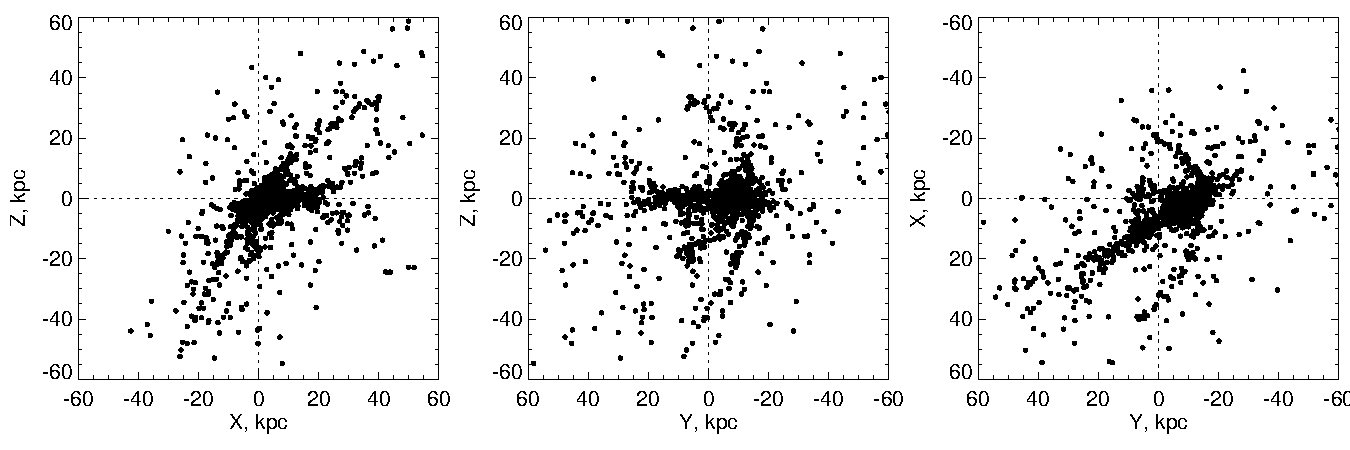
\includegraphics[width=0.95\textwidth]{orphan_paper_xyz.pdf}
  \caption[]{The Magellanic Clouds in Gaia DR2. Only stars with
    parallax $\varpi<0.2$ mas are used. {\it Left:} Logarithm of the
    density of the outer LMC stars in $G$ vs $G_{\rm BP}-G_{\rm RP}$
    space (all de-reddened). {\it Middle Left:} Logarithm of the
    density of stars in the Galactic foreground near the Clouds
    (i.e. stars above $|b|=5^{\circ}$ and between $20^{\circ}$ and
    $60^{\circ}$ from the LMC, excluding an area with a $10^{\circ}$
    radius around the SMC). {\it Middle Right:} The difference of the
    CMD densities shown in the first two panels. Apart from some minor
    contamination at faint $G$ and red $G_{\rm BP}-G_{\rm RP}$, the
    strongest over-density is that corresponding to the LMC's red
    giant branch. The black-white dashed line shows the CMD mask used
    to select the likely LMC (and SMC) giants. {\it Right:} Logarithm
    of stellar density in PM space. In addition to the CMD selection
    shown in the middle panels, we select stars within $15^{\circ}$
    ($10^{\circ}$) of the LMC's (SMC's) center and with $G_{\rm
      BP}-G_{\rm RP} > 1.3$. Black lines outline the PM selection box
    used to improve purity of the tracer population. Note that the
    foreground contribution within the PM box is $<1\%$.}
   \label{fig:selection}
\end{figure*}
%

It so happened that the most striking example of a nearby binary
interaction was only just being discovered at the time of the writing
of \citet{Toomre1972} and hence could not be included in their
analysis. \citet{Wannier1972} and \citet{Kuilenburg1972} detected long
streams of HI in the Southern sky, and some two years later these were
shown to connect to the Magellanic Clouds by
\citet{Mathewson1974}. The Magellanic Stream (MS, as it is known
today) has since been mapped across the sky \citep[see
  e.g.][]{Putman2003,Nidever2008,Nidever2010} and is today
unambiguously demonstrated to have originated in the interaction
between the Large and the Small Clouds \citep[LMC and
  SMC,][]{Besla2007, Besla2010, Diaz2011, Diaz2012}. While the stellar
counterpart to the MS is yet to be discovered, the last two years have
seen a marked increase in the number of reported detections of low
surface-brightness stellar sub-structure in the vicinity of the Clouds
\citep[see
  e.g.][]{Mackey2016,Belokurov2016,Belokurov2017,Deason2017,Pieres2017,Mackey2018,Nidever2018}. In
particular, \citet{Mackey2016,Mackey2018} concentrate on the
perturbations in and around the LMC's stellar disc. They uncover a
wealth of sub-structure, some of which (such as the long stream-like
feature in the North of the LMC) they tentatively attribute to the
tidal influence of the MW \citep[][]{Mackey2016}. They also
detect prominent stellar debris over-densities in the Southern parts
of the LMC and put forward two formation scenarios: one to do with the
disruption of the LMC's disc and one linked to the episodic stripping
of the SMC \citep[see also][who argued for the importance of repeated
  interactions with the SMC]{besla_etal_2016}.

%
\begin{figure*}
  \centering
  \includegraphics[width=0.9\textwidth]{orphan_paper_selection.pdf}
  \caption[]{Kinematics of the selected RG stars. {\it Left Column:}
    Median values of $\mu_{\rm L}$ (top) and $\mu_{\rm B}$ (bottom) PM
    components in each pixel of $L_{\rm MS}, B_{\rm MS}$. {\it Right
      Column:} PM dispersion (around the median) maps corresponding to
    the median motion maps shown in the left column. Note that PM
    variations mapped here are much larger than the Gaia PM
    systematics of $\sim$0.04 mas year$^{-1}$ \citep[see][]{Arenou2018}.}
   \label{fig:vel}
\end{figure*}
%


%
\begin{figure*}
  \centering
  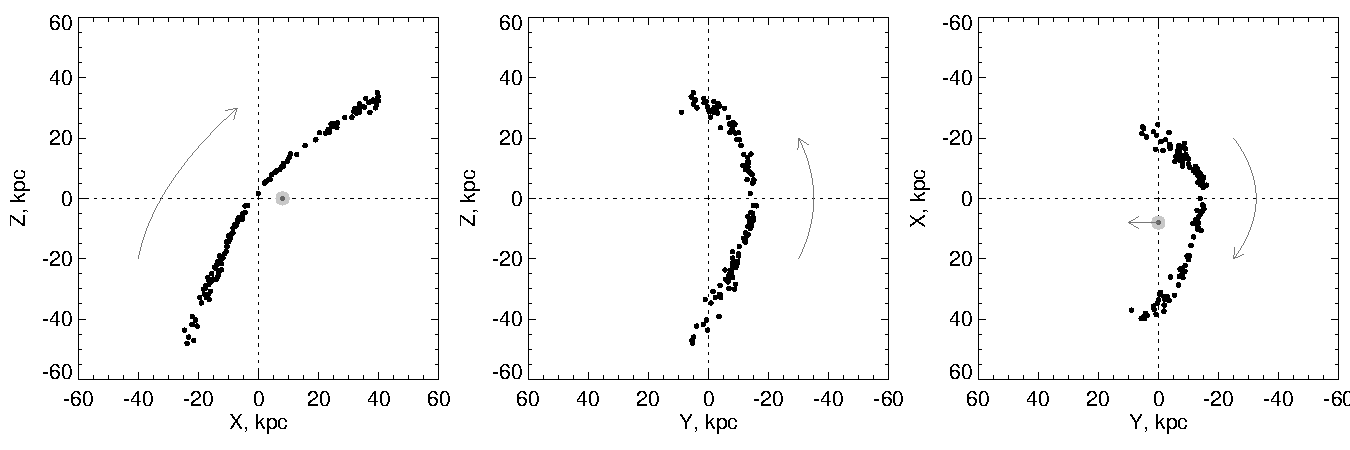
\includegraphics[width=0.97\textwidth]{orphan_paper_xyz_members.pdf}
  \caption[]{ {\it Left:} Map of the distribution of the total dust
    extinction centered on the LMC as measured by \citet{SFD} {\it
      Middle:} Density of the candidate RGB stars selected using cuts
    illustrated in Figure~\ref{fig:selection} and described in the
    main text. Filled black circle marks the location of the Carina
    dwarf spheroidal galaxy. {\it Right:} Same as Middle but saturated
    at lower density levels. Number of stars per square degree
    corresponding to the white (low density) and black (high density)
    is given in the title.}
   \label{fig:map}
\end{figure*}
%

In this Letter, we use a combination of Gaia's (Data Release 2, or
GDR2) photometry and astrometry to produce an uninterrupted panorama
of the Magellanic Clouds. We focus on the density fluctuations between
10 and 30 degrees away from the LMC's centre. While our maps do not
attain the same level of detail achievable using deep imaging with
instruments such as DECam, they help to fill in the gaps in the
Magellanic puzzle. Moreover, Gaia's astrometry has the
unprecedented power to remove the bulk of the intervening MW's
disc population and thus extend the study of the Clouds to regions
not accessible even with the deepest imaging surveys.

%Specifically, we demonstrate that two long and narrow tidal arms exist
%in the Northern and Southern outskirts of the LMC's disc, most likely
%produced as a result of the combined effect of the MW tides and the
%interaction with the SMC during its most recent passage near the Large
%Cloud.

\section{Gaia DR2 view of the Magellanic Clouds}

In what follows we use the photometry and astrometry provided as part
of the Data Release 2 \citep[][]{Brown2018} of the Gaia mission
\citep[][]{Prusti2016}. We correct the $G, G_{\rm BP}$ and $G_{\rm
  RP}$ magnitudes for the effects of extinction using the first two
terms in the Equation 1 of \citet{Babusiaux2018} and the dust maps of
\citet{SFD}. Additionally, we remove the foreground dwarf stars from
our sample by culling all objects with parallax $\varpi>0.2$ mas and
exclude stars with Galactic latitudes $|b|<5^{\circ}$. We note that
this is not the first attempt to use GDR2 to study the LMC (and the
SMC): the kinematic view of the inner portions of each Cloud can be
found in \citet{Helmi2018}, while \citet{Vasiliev2018} presents the
first results of dynamical modelling of the inner LMC.

Figure ~\ref{fig:selection} shows the behavior of stars with
$\varpi<0.2$ mas in the vicinity of the Clouds in color-magnitude and
proper motion (PM) spaces. More precisely, the left panel displays the
density of stars within 12 degrees of the LMC's center in $G$ vs
$G_{\rm BP}-G_{\rm RP}$ plane (Hess diagram). Here we assumed that the
center of the dwarf is located at $\alpha, \delta =
80.89375^{\circ},-69.7561^{\circ}$. The CMD signal of the LMC can be
compared to that of the Galactic foreground shown in the second panel
of the Figure. We give the difference of the two in the third
panel. In this Hess difference plot, the LMC's Red Giant Branch (RGB)
and the Red Clump (RC) are easily discernible (their envelope is
traced by black-and-white dashed line). Note that the tip of the RGB
runs horizontally (i.e. at constant $G$) for colors redder than
$G_{\rm BP}-G_{\rm RP} \simeq 2$. While the RC is the most densely
populated CMD feature, it is also the one that suffers the highest
Galactic foreground contamination, especially at $G_{\rm BP}-G_{\rm
  RP}<0.9$ and $G>19$. Therefore, to select the likely Magellanic
stars we choose objects with $\varpi<0.2$ mas that fall within the CMD
mask (broad enough to accommodate the heliocentric distance range
across the Magellanic system) shown in panels 2 and 3 of
Figure~\ref{fig:selection} and have $G_{\rm BP}-G_{\rm RP}>0.9$ and
$G<19$. Finally, to further improve the purity of our selection we
apply PM cuts chosen to delineate the motion of genuine LMC
and SMC stars as shown in the fourth (rightmost) panel of the
Figure. Here, stars within 15$^{\circ}$ of the LMC and 7$^{\circ}$ of
the SMC are shown in $\mu_{\rm L}, \mu_{\rm B}$ PM space
aligned with the gaseous MS \citep[see][for the definition of the
  $L_{\rm MS}, B_{\rm MS}$ coordinate system]{Nidever2008}. Note that
to clarify the over-densities corresponding to the Clouds, for this
panel only, we additionally limit the stars to those with $G_{\rm
  BP}-G_{\rm RP}>1.3$.

The density of the likely Magellanic RGB candidate stars selected
using a combination of parallax, $|b|$, CMD and PM cuts
described above is shown in Figure~\ref{fig:map}. The same density map
is displayed twice, in the middle and right panels of the Figure,
albeit with different saturation levels to help study features across
a wide range of surface brightness values. Note that even at
astonishingly low Galactic latitudes, $|b|<10^{\circ}$, very little
disc contamination is visible thanks to the power of Gaia's
astrometry. Comparing the stellar density patterns in panels 2 and 3
with the dust distribution shown in panel 1, we conclude that the
only noticeable correlation between the two maps can be seen in the
very cores of each Cloud, where the star counts are depleted by high
values of extinction. Figure~\ref{fig:map} reveals an intricate and
spatially extended system of narrow stream-like structures emanating
from the LMC's disc. A large portion of the Northern arm was already
discussed in \citet{Mackey2016}, where it was traced out to
$\sim20^{\circ}$ away from the LMC's center. Here we show that this
structure continues to higher $L_{\rm MS}$ for (at least) some
$5^{\circ}$ to $10^{\circ}$, passing right under the Carina dwarf,
where, as pointed in \citet{Mackey2016}, the LMC's stars have been
detected before \citep[see][]{Majewski2000, McMonigal2014}. In the
Southern regions of the LMC, a more complicated web of sub-structures
can be seen. There are two ``claw''-like over-densities, identified as
``Substructure 1'' and ``Substructure 2'' in
\citet{Mackey2018}. Curiously, in the maps presented here,
``Substructure 2'' appears to be curving clockwise, continuing as far
as $(L_{\rm MS}, B_{\rm MS})=(10^{\circ},-5^{\circ})$. One of the most
striking new features is a thin stellar stream which appears to be
connecting to the SMC at around $L_{\rm MS}\sim-8^{\circ}$. This
narrow tail, one of the longest structures discussed here, wraps
around the Southern edge of the LMC's disc, tracing an arc of
$\sim$90$^{\circ}$ in clockwise direction. As gleaned from
Figure~\ref{fig:map}, the LMC appears to have two long arms, one in
the North and its counter-part in the South.

%
\begin{figure*}
  \centering
  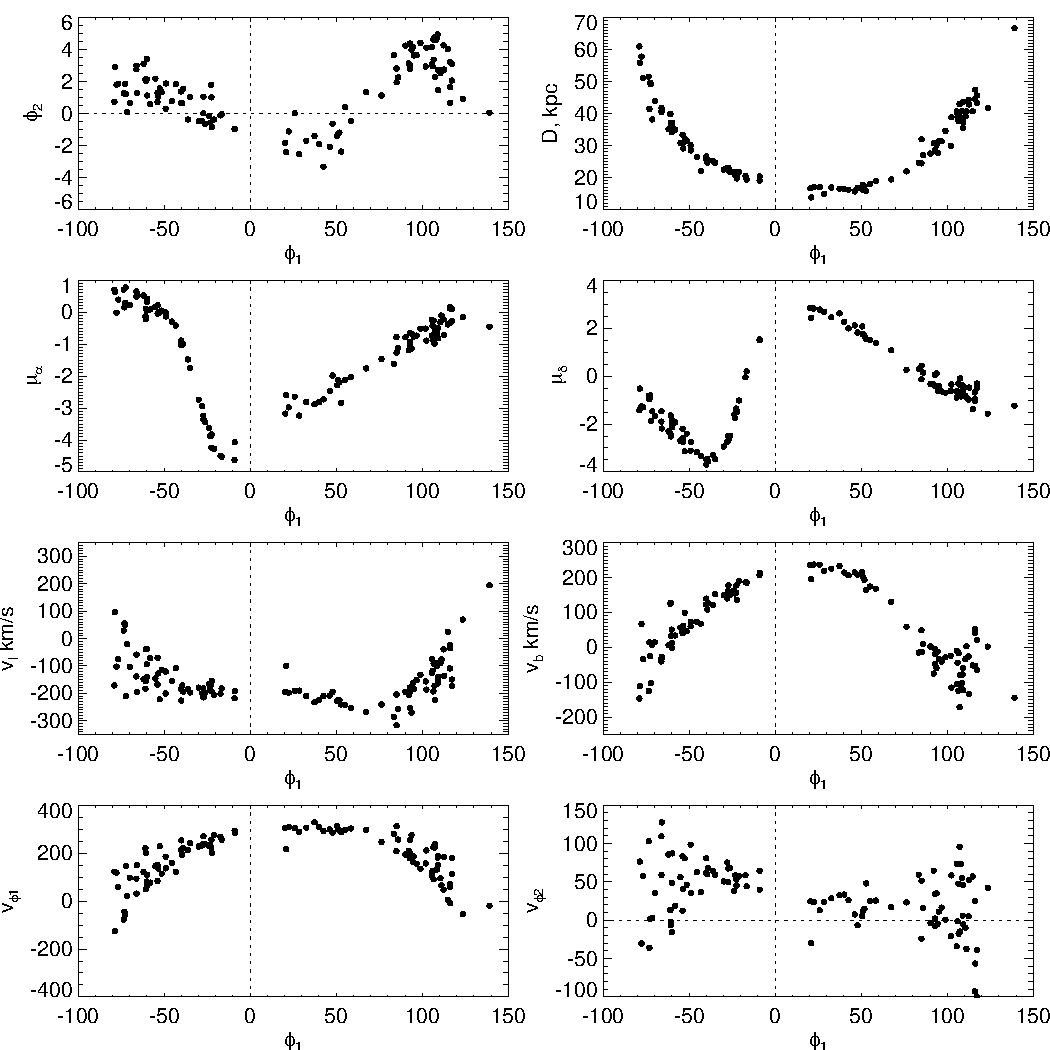
\includegraphics[width=0.9\textwidth]{orphan_paper_phi1_members.pdf}
  \caption[]{Kinematics of the selected RG stars. {\it Left Column:}
    Median values of $\mu_{\rm L}$ (top) and $\mu_{\rm B}$ (bottom) PM
    components in each pixel of $L_{\rm MS}, B_{\rm MS}$. {\it Right
      Column:} PM dispersion (around the median) maps corresponding to
    the median motion maps shown in the left column. Note that PM
    variations mapped here are much larger than the Gaia PM
    systematics of $\sim$0.04 mas year$^{-1}$ \citep[see][]{Arenou2018}.}
   \label{fig:vel}
\end{figure*}
%

To clarify the origin of the stellar over-densities described above,
Figure~\ref{fig:vel} gives the PMs of the selected LMC's candidate RGB
stars. Note that these PMs have been corrected for the Solar reflex
assuming a constant heliocentric distance of 49.9 kpc. The pattern of
the median PM values (left column of the Figure) across the inner
$10^{\circ}$ (smaller dashed circle) is dominated by the gradient
associated with the Cloud's rotation \citep[see
  also][]{Vasiliev2018}. Note, however, that the stellar motions
preserve coherence well outside the central LMC. More fascinating
still, all of the narrow arm-like features at distances beyond
$\sim15^{\circ}$ also display coherent systematic motions. Overall,
the kinematics of the Northern and Southern arms resembles that of the
outer LMC's disc but off-set in orbital phase. Note that the bulk of
the Southern sub-structure shares the PM of the LMC. This is
especially evident in the lower left panel, where the stellar streams
have colors from green to red, similar the LMC's disc, while the SMC
is dark blue. While not the main focus of this Letter, it is worth
commenting briefly on the PM pattern of the SMC. According to
Figure~\ref{fig:vel}, the SMC's systemic motion is in the direction
away from the LMC, i.e. towards negative $L_{\rm MS}$ and negative
$B_{\rm MS}$, consistent with previous measurements \citep[see
  e.g.][]{kallivayalil_lmc_pm}. Also visible are clear proper motion
gradients, whose direction is roughly aligned with the line connecting
the centers of the two Clouds. While this gradient could be modelled
as an intrinsic rotation signal \citep[see e.g.][]{Helmi2018}, we
suggest it could also be the result of the strong tidal stretching of
the SMC by the LMC \citep[see also][]{Zivick2018}.


The right column of the Figure presents dispersions around the median
values of PM components $\mu_{\rm L}$ and $\mu_{\rm B}$ for each pixel
of $L_{\rm MS}$ and $B_{\rm MS}$. Strong perturbations of the inner
LMC's disc have recently been reported in the literature
\citep[see][]{Choi2018}, but here, we offer a much more complete map
of kinematically cold (blue) and hot (red) regions across the entire
Cloud. The regions of elevated dispersion are clearly different for
the longitudinal and latitudinal PM components. For
$\mu_{\rm L}$, the hottest region is on the rim of the LMC's disc
facing the SMC and in between the Clouds, where one naturally expects
a mixture of stars from both dwarfs. In $\mu_{\rm B}$, there are two
extended regions with high PM dispersion, one in the North
and one in the South, located radially inward from the locations of
each arm. The arms themselves are distinctly cold as judged by their
dark blue color.

\section{Simulations, Caveats and Conclusions}

In order to investigate how the MW and SMC affect the LMC's disc and
whether they can induce the spiral features shown in Figure
\ref{fig:map}, we have run a series of simulations in the spirit of
\cite{Toomre1972}. In particular, we simulate the disc of the LMC as a
series of particles in concentric rings which are initially on
circular orbits. While this ignores the initial non-circular motions,
it captures the overall behavior of the disc over the relatively short
timescales considered here. The system is then evolved in the presence
of the MW and the SMC. We model the LMC's potential as a Hernquist
profile \citep{hernquist_profile} which satisfies the rotation curve
measurement at a radius of 8.7 kpc from \cite{vandermarel_lmc} (for
each LMC mass, the scale radius is fixed by this constraint). The
initial orientation and rotation sense of the LMC are chosen to match
the observations from \cite{vandermarel_lmc}. The SMC is also modelled
as a Hernquist profile satisfying the rotation curve measurement at a
radius of 3 kpc from \cite{staminirovic_smc_mass}. The MW is modelled
as the 3-component potential, \texttt{MWPotential2014}, from
\cite{galpy}. Starting from their present day positions, the LMC and
SMC are rewound for 1 Gyr (in the presence of each other and the MW),
at which point particles are placed on circular orbits around the
LMC. For each simulation, we place 5000 particles on 50 separate
concentric circles with radii evenly spaced from 1 to 20 kpc. The
simulation is then evolved to the present. For the LMC's present day
position and velocity, we use a distance of $49.97 \pm 1.126$ kpc
\citep{pietrzynski_lmc_dist}, a radial velocity of $-262.2\pm3.4$ km/s
\citep{vandermarel_lmc_rv}, and PMs of $(\mu_\alpha \cos \delta,
\mu_\delta) = (1.91\pm 0.02,0.229\pm0.047)$ mas/yr
\citep{kallivayalil_lmc_pm}. For the SMC, we use a distance of
$62.1\pm1.9$ kpc \citep{graczyk_smc_distance}, a radial velocity of
$145.6\pm0.6$ km/s \citep{harris_smc_vel}, and PMs of
$(\mu_\alpha \cos \delta, \mu_\delta) = (0.772\pm
0.063,-1.117\pm0.061)$ mas/yr \citep{kallivayalil_lmc_pm}. For each
choice of the LMC and SMC masses and scale radii, we sample their
present day position and velocity and simulate 100 realizations to
explore the variety of outcomes.

In Figure \ref{fig:sim_multi} we isolate the effect of the MW
(left-most column) and the SMC (middle two columns) on the LMC. The
two rows show two different realizations of the LMC and SMC's present
day position and velocity. The top row shows an LMC with a closer
encounter with the SMC ($r_{\rm peri} \sim 10$ kpc), while the bottom
row shows a more distant encounter ($r_{\rm peri} \sim 15$ kpc). The
tidal field of the MW is primarily responsible for bending the
Northern half of the LMC, similar to what was found in $N$-body
simulations in \cite{Mackey2016}, and creates a spiral arm feature
similar in position and orientation to what it seen in the data. The
SMC can create one or two spiral arms, depending on how strong of an
interaction it has with the LMC during its most recent
pericenter. While this is in seeming contradiction to the results of
\cite{Toomre1972}, we stress that we are observing the LMC disc only
$\sim 150$ Myr after its most recent passage with the SMC and that it
takes time for the spiral features to form. If the LMC was simulated
for longer, the second spiral would form in the lower panel of Figure
\ref{fig:sim_multi}. Interestingly, we find that the SMC creates a
strong spiral arm in the South which matches the observed Southern
stream. We found that changing the SMC mass from $5\times 10^9
M_\odot$ to $10^{10} M_\odot$ resulted in only a modest change in the
spiral features. Our simulations do not contain the ``claw''-like
features visible in the data in the Southern parts of the LMC. We
conjecture that these density features are remnants of much earlier
interactions between the two Clouds. The fourth column of the figure
shows the effect of both the MW and the SMC. This
demonstrates that their combined effect is needed to create the two
spirals observed in the LMC. It also illustrates how a close encounter
with the SMC can truncate the Western portion of the LMC's disc (top,
second from the right panel) similar to what it seen in the
data. Taken together, this shows that morphology of the LMC's disc and
the associated spiral structure can be used to reveal its rich
dynamical history.

In a similar vein, we also explore the effect of the LMC's mass on its
morphology in Figure \ref{fig:sim_multi}. While the first four columns
show a $2\times 10^{10}M_\odot$ LMC, the final column shows a $2\times
10^{11} M_\odot$ LMC.  Note that the final column should be compared
with the fourth column since these have the same setup.  As the LMC
mass is increased, we find that the LMC is deformed less by the
MW. This is because the increased LMC mass results in a larger tidal
radius and hence a larger region where the effect of the MW is
negligible. Interestingly, only the lowest mass LMC we consider
($2\times 10^{10} M_\odot$) can match the tightly wound spiral seen in
the North (see Fig. \ref{fig:map}). Since this mass is only slightly
higher than the mass constraint within 8.7 kpc from
\cite{vandermarel_lmc}, this could suggest that the LMC has already
been significantly stripped. However, we stress that these simulations
are only meant to be the first step in showing that the morphology
(including spirals) of the LMC's disc can provide useful constraints
on the properties of the LMC, SMC, and on the tidal effect of the
MW. With this aim in mind, the rich PMs in Figure
\ref{fig:vel} will also be useful in future modelling efforts.

In summary, we have used the exquisite data from Gaia DR2 to
unveil a global view of the perturbations to the LMC's disc. In
particular, there are two clear spiral features, as well as some complex
substructure to the South of the LMC (see Fig. \ref{fig:map}). While
some of this structure was seen before
\citep[e.g.][]{Mackey2016,Mackey2018}, the uninterrupted view afforded
by Gaia allows us to better understand how these features
arose. We simulated the combined effect of the MW and SMC on
the LMC's disc and found that both are important for creating the
spiral features seen in the data. Namely, the MW is responsible
for deforming the Northern part of the LMC while the most recent
passage of the SMC creates the strong spiral feature in the South. A
close passage with the SMC can also truncate the Western side of the
LMC's disc. Finally, we showed that the distant Magellanic Red
Giants detected here can be used to map out the LMC's mass distribution at
unprecedentedly large distances.

\section*{Acknowledgments}

We thank Michael for illuminating discussions. The research leading to
these results has received funding from the European Research Council
under the European Union's Seventh Framework Programme (FP/2007-2013)
/ ERC Grant Agreement n. 308024. This research was started at the NYC
Gaia DR2 Workshop at the Center for Computational Astrophysics of the
Flatiron Institute in April 2018 and made use of data from the
European Space Agency mission Gaia (http://www.cosmos.esa.int/gaia),
processed by the Gaia Data Processing and Analysis Consortium (DPAC,
http://www.cosmos.esa.int/web/gaia/dpac/consortium). Funding for the
DPAC has been provided by national institutions, in particular the
institutions participating in the Gaia Multilateral Agreement.

\bibliography{references}

\label{lastpage}

\end{document}

